\documentclass[conference]{IEEEtran}
\IEEEoverridecommandlockouts
% The preceding line is only needed to identify funding in the first footnote. If that is unneeded, please comment it out.
\usepackage{cite}
\usepackage{amsmath,amssymb,amsfonts}
\usepackage{algorithmic}
\usepackage{graphicx}
\usepackage{textcomp}
\usepackage{romannum}
\usepackage{enumitem}   


\def\BibTeX{{\rm B\kern-.05em{\sc i\kern-.025em b}\kern-.08em
    T\kern-.1667em\lower.7ex\hbox{E}\kern-.125emX}}
\begin{document}

\title{CS6290: Reading Summary \Romannum{4}}

\author{\IEEEauthorblockN{Yang Ji}
\IEEEauthorblockA{ID:\ 56064832 \\
yangji@comp.hkbu.edu.hk \\
Dept.\ of Computer Science}
}

\maketitle

\section{Summary of Paper \cite{lu2018zebralancer}}

\subsection{Problem Statement}
This paper implements a crowdsourcing system atop public blockchain, namely ZebraLancer, which achieves the fair exchange without any trusted third party.
%
In particular, this system tries to resolve two general privacy challenges: (1) the tension between blockchain transparency and data confidentiality (2) the tension between anonymity and accountability. 

\subsection{Problem Significance}
In practice, the reduction of the reliance on a trusted third-party is desirable due to the following reasons:
%
\begin{itemize}
    \item The arbiter might misbehave for his/her own self-interets. 
    \item Current crowdsourcing systems are biased on requestors over workers.
    \item Single point failure.
    \item Massive privacy leakage. For example, Uber tried to hide the fact of data leakage in 2016.  
\end{itemize}
 
\subsection{Preliminaries}
\subsubsection{Crowdsourcing System}
Crowdsourcing is a common business model which empowers open and wide collaboration over the Internet with lower cost and high scalability.
%
In the classical crowdsourcing system, requesters need to adopt reasonable incentive policies to motivate workers' participation.
%
To ensure the fair exchange, a trusted third party is usually used to host crowdsourcing tasks and help resolve the dispute.
%

\subsection{State of the Art}
To solve the above problems, we could employ open blockchain to remove a trusted third-party and realize a decentralized crowdsourcing system.
%
Blockchain has many valuable features which can help remove the trusted arbiter safely. 
%
Firstly, open blockchain could be viewed as a distributed, transparent and immutable public 'bulletin board'.
%
Any data can't be modified and accessible to the public.
%
Then pre-defined consensus protocol ensures reliable message deliveries via the untrusted Internet. 
%
What's more, smart contract can faithfully execute all computations and message deliveries.
%
Requesters can deploy tasks in the form of smart contract into the blockchain and workers can submit their answers to the corresponding addresses through transactions.

However, public blockchain also brings about many new problems which are not shown before at all.
%
For one thing, transparency violates data privacy directly.
%
For example, workers' submitted answers are exposed to other peers who can simply copy them and form free-riding attacks.
%
For another thing, totally transparency could cause misbehaviors by colluded counterfeit identities.

%\begin{figure}[ht]
%    \centering
%    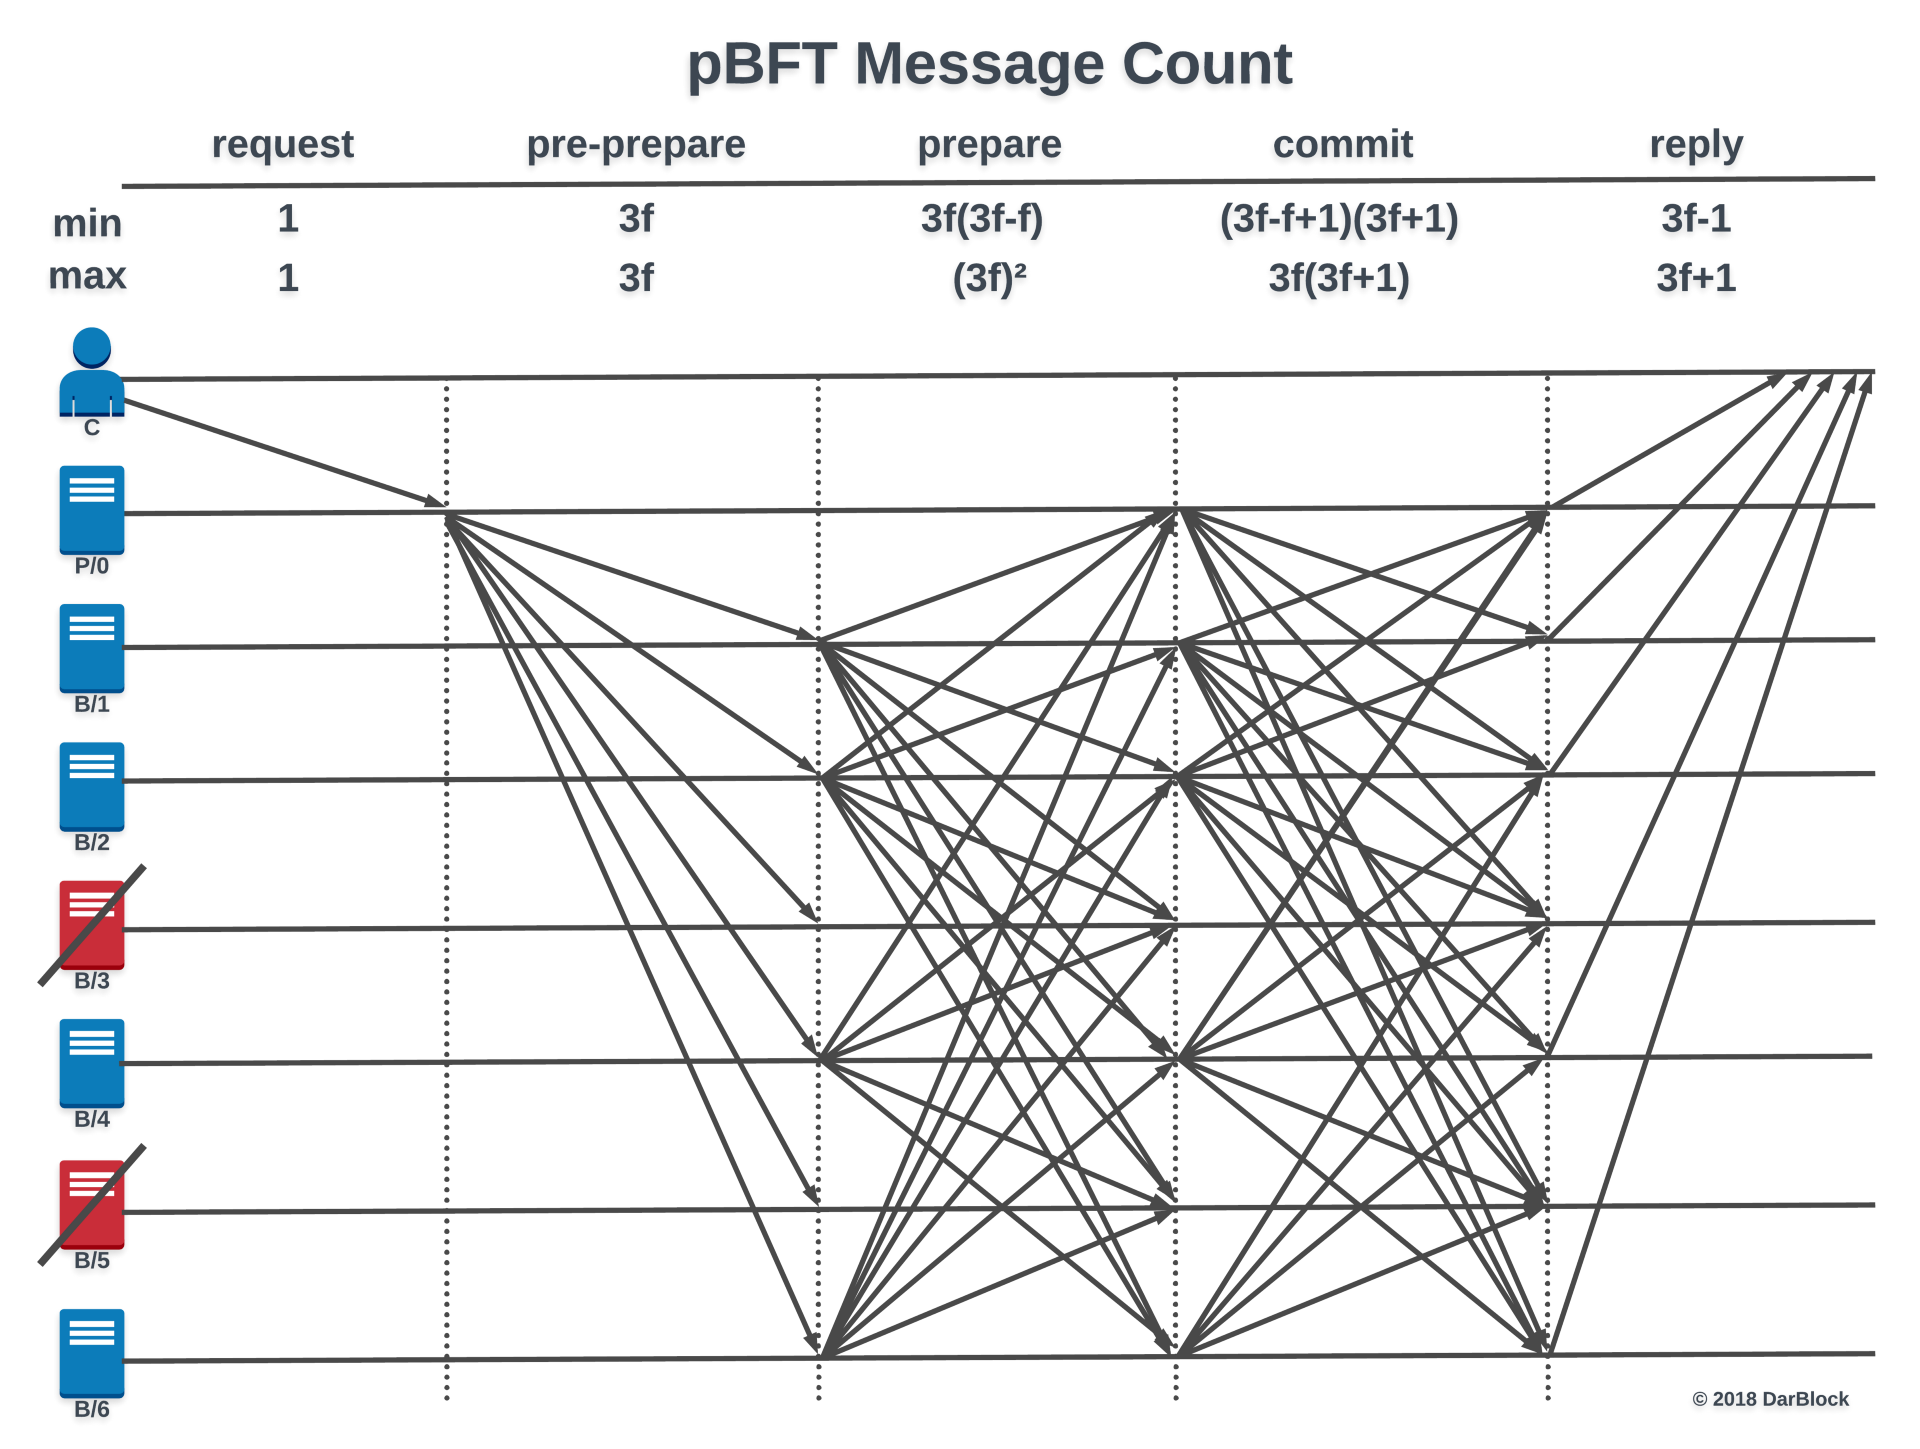
\includegraphics[width= 0.95\linewidth]{fig/PBFT.png}
%    \caption{Normal Case Operations}
%    \label{pbft}
%\end{figure}

\subsection{Contributions}
The model of data crowdsourcing consists of four components:
\begin{itemize}
    \item \textbf{Registration Authority (RA).} All users including requesters and workers must obtain unique credentials from RA which are bound to their true identities.
    \item \textbf{Authenticated Requesters.} Users who issue crowdsourcing tasks.
    \item \textbf{Authenticated Workers.} Users who help resolve launched tasks.
    \item \textbf{Platform.} This platform is used to fulfill the fair exchange by faithfully executing requesters' pre-defined incentive policies. In this paper, this platform is actually Ethereum. 
\end{itemize} 

It is worth nothing that RA is introduced to prevent users from misusing anonymity. 
%
The authors define existing problems of decentralized crowdsourcing systems as follows: 
(1) \textbf{Data Confidentiality:} Any information of the content of submitted answers shouldn't be accessible to the public.  
(2) \textbf{Anonymity:} This property ensures that we can't link a submission or joined tasks to a particular worker/requester.

To settle the first treat, the authors enforce the workers to encrypt their submitted answers under the requester's public key, which means only the requester of this task could decrypt these answers.
%
But this leads to a new problem for smart contract because encryption prevents smart contract from enforcing the incentive policy and requesters can't put their secret keys into the smart contract.
%
In this paper, the authors leverage a zero-knowledge tool called zk-SNARK to realize a proving and verifying mechanism to enforce the fairness.
%
In more detail, the requester need to generate a zero-knowledge proof of his/her faithful computation and smart contract could verify this succinct proof expediently.

For the second security issue, the authors create a common-prefix-linkable anonymous authentication scheme to keep sure that users could submit anonymous answers once for one task.
%
Once a particular worker submits his/her answer more than once, smart contract can link these submissions together ,which could prevent the misuse of anonymity efficiently.
%
The detailed solution is to append a prefix string to every submission which corresponds to each task.

\subsection{Remaining Questions}
Firstly, I think requesters don't need to hash their secret keys in the head which seems useless in the whole scheme construction.
%
Secondly, the experiment results show that incentive policy is quite simple which only costs 10ms for verification.
%
Thirdly, zkSNARK needs a trusted setup phase to generate proving and verifying key ,which means more work for Registration Authority.


\section{Summary of Paper\cite{croman2016scaling}}

\subsection{Problem Statement}
This paper tries to explain and analyze the possible solutions on efficiently scaling current blockchain systems, including parameter tuning and reconstruction of a scalable blockchain.

\subsection{Problem Significance}
As a cryptocurrency system, current blockchain needs to improve the capacity of dealing with transactions.
%
Take Bitcoin as an example.
%
In Bitcoin network, miners need 10 minutes or more to publish a new block and confirm 7 transactions per second at most.
%
In comparison, visa credit card which is a mainstream payment processor can deal with about 2000 transactions per second.
%
The huge gap between blockchain system and traditional payment processor incentivizes blockchain developers to rethink how to scale up network efficiently.

\subsection{State of the Art}
This article reviews the current technologies on scaling blockchains from two perspectives.
%
For one thing, reparameterization of block size and intervals can be viewed as a temporary and limited approach to more scalable blockchains.
%
For another thing, a radical reconstruction of blockchain systems might be the fundamental solutions on scaling up the throughput of blockchains.  
%
Before concluding the analysis of these approaches, I firstly will introduce some preliminaries on network measurement.

\subsection{Preliminaries}

\subsubsection{Maximum Throughput} It describes the maximum quantity of transactions which blockchains could confirm. In general, it is mainly adjusted by the block size and inter-block intervals.

\subsubsection{Latency} Based on the pre-defined consensus protocol, a new block containing variety of transactions needs to wait for around 10 minutes to be confirmed determinately.

\subsubsection{Bootstrap Time} It records the time that a newly joint node needs to prepare for validating the current network status. For Bitcoin, this time is roughly 4 days.

\subsubsection{Cost per Confirmed Transaction (CPCT)} CPCT represents the average cost of confirming a new transaction in the form of USD. 
%
In more details, the cost could derive from the following four sources: (i) Mining (ii) Transaction validation (iii) Bandwidth (iv) Storage.

\subsubsection{X$\%$ Effective Throughput} Here, authors define this concept as (block size) / (X$\%$ block propagation delay) which means that (100-X)$\%$ of the nodes in the network are unable to receive blocks correctly.


\subsection{Contributions}

\subsubsection{Parameter Tuning} 
To be more precise, we could adjust the block size (decides to contain how many transactions in each block) and inter-block intervals actually. 
%
However, we can't increase the block size and reduce intervals infinitely.
%
In order to keep the property of decentralization in the whole system, X$\%$ effective throughput should be at a relatively high level.
%
In other words, if X is fixed on 90, what we could do is just to increase the block size or reduce the inter-block intervals unilaterally.
%
And there exists two main limits on current overlay network:

\begin{itemize}
    \item \textbf{Throughput Limit.} Assume that the inter-block interval is 10 minutes, the block size should not exceed 4MB which can support up to 27 transactions per sec.
    \item \textbf{Latency Limit.} In order to thoroughly employ the bandwidth of the network, the block intervals should be smaller than 12 second.
\end{itemize}

\subsubsection{Hierarchical Design of a Scalable Blockchain}
The paper concludes this design from five perspectives: Network, Consensus, Storage, View and Side planes.

\begin{itemize}
    \item \textbf{Network Plane.} The main reason for latency in Bitcoin is the duplex transmissions at the node level. 
    Nodes need to validate local transactions before publishing this new block.
    A set reconciliation protocol and a centralized, high-speed relay network specially for miners' communication can be possible approaches to this problem.
    \item \textbf{Consensus Plane.} This network plane is aimed to achieve the consensus in the whole network. 
    Many alternatives can substitute PoW protocol to improve the network performance, like GHOST, PoS et al.
    It is worth nothing that sharding (splitting up the problem of consensus) or delegation of trusted and hierarchical sidechains might be a potential solution.
    \item \textbf{Storage Plane.} It provides the storage service for the consensus plane. Operations might include writing, deleting and reading.
    \item \textbf{View Plane.} Authors put forward two potential approaches including nodes replication and data outsourcing.
    \item \textbf{Side Plane.} Side plane provides a off-chain method to realize the payment in a more efficient manner. 
    Through pre-established channels, it solves the inherent problems by introducing a centralized approach.
\end{itemize}

\subsection{Remaining Questions}
Although with these potential solutions on scaling up the blockchain system, it still remains a huge challenge of coordinating the whole system in an efficient manner.
%
What's more, how to persuade the majority to accept a hard fork is another difficult task for the community. 

\bibliographystyle{IEEEtran}
\bibliography{references}


\end{document}
